\section{Background}

X-rays are a type of ionizing electromagnetic radiation with typical energies in the \unit{\kilo\electronvolt} range. Their
production inside an X-ray tube relies on the electrostatic acceleration of electrons which then interact with the anode material. The main
mechanisms for the emission of energetic photons are the continuous bremsstrahlung resulting from electron deceleration as well as a
discrete component emitted after penetration of the inner atomic shells \cite{McMorrow_2011_1, McMorrow_2011_2}.



\subsection{Refractive index}

In classical ray optics, the laws of reflection and refraction are
\begin{align}
	\theta_i = \theta_r \: , && n_1 \cos\theta_i = n_2 \cos\theta_t \: ,
	\label{eqn:snell}
\end{align}
where $n_1$ and $n_2$ are the refractive indices of the two media and $\theta_i, \theta_r, \theta_t$ are the angles of incidence, reflection
and transmission as shown in Figure \ref{fig:fresnel}.

\begin{figure}[H]
	\centering
	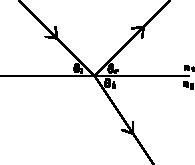
\includegraphics[width=0.33\textwidth]{content/graphics/fresnel.pdf}
	\caption{Depiction of reflection and refraction of light rays on a smooth surface.}
	\label{fig:fresnel}
\end{figure}

For X-rays, the refractive index can usually be written as
\begin{equation*}
	n_2 \equiv n = 1 - \delta \pm i\beta \: ,
\end{equation*}
with the extinction coefficient $\beta > 0$ measuring the exponential absorption and a small correction $\delta > 0$ for the dispersion.
The choice of $\pm$ depends on the sign convention for the wave vector. From $1 - \delta < 1$ further follows that the phase velocity
of X-rays can exceed the speed of light in vacuum $c$. Because information travels at the group velocity, this does not violate special
relativity. Assuming air or vacuum as the surrounding medium, one can set
\begin{equation*}
	n_1 \equiv 1 \: ,
\end{equation*}
resulting in a transition from an optically thick to a thin medium. Accordingly, total reflection occurs for small angles
$\theta_i < \theta_c,$ with
\begin{equation*}
	\theta_c = \arccos n
\end{equation*}
defining the critical angle. Proceeding in the small angle approximation, one can expand
\begin{equation*}
	\cos\theta \cong 1 - \pfrac{1}{2} \theta^2
\end{equation*}
to second order. Rewriting Snell's law \eqref{eqn:snell} as
\begin{equation*}
	1 - \pfrac{1}{2} \theta_i^2 \cong n \left( 1 - \pfrac{1}{2}\theta_t^2 \right) = (1 - \delta \pm i\beta) \left( 1 - \pfrac{1}{2}\theta_t^2 \right)
	\cong 1 - \delta \pm i\beta - \pfrac{1}{2}\theta_t^2
\end{equation*}
yields the relationship
\begin{equation}
	\theta_t \cong \sqrt{\theta_i^2 - 2\delta \pm 2i\beta} \: ,
	\label{eqn:angles}
\end{equation}
where products of $\delta, \beta, \theta_t \ll 1$ are ignored in the last step. Similarly, one identifies
\begin{equation*}
	\theta_c \cong \sqrt{2\delta \mp 2i\beta}
\end{equation*}
by setting $\theta_t = 0$ in \eqref{eqn:angles}. Noting $k \rightarrow nk$ for the wave propagating in the medium,
\begin{equation*}
	e^{\pm i nkz} = e^{i(1 - \delta)kz} e^{-\beta kz}
\end{equation*}
and from this
\begin{align}
	\delta &= \pfrac{2\pi \rho_e r_e}{k^2} \: , \label{eqn:dispersion} \\
	\beta &= \pfrac{\mu}{2k} \: , \label{eqn:extinction}
\end{align}
relate $\delta, \beta$ to the electron density $\rho_e$ and the absorption coefficient $\mu$ via the electron radius $r_e = e^2 / m_e c^2$
and $k = 2\pi / \lambda$ \cite{McMorrow_2011_3}.



\subsection{Fresnel coefficients}

By decomposing any electromagnetic wave into linearly polarized components with the electric field oscillations orthogonal (s-polarization) or
parallel (p-polarization) to the plane of incidence, one can derive Fresnel's formulae due to continuity of the tangential field component. For
the amplitude ratio of reflected to incident ray, this reads as
\begin{equation*}
	r_s = \pfrac{\sin\theta_i - n\sin\theta_t}{\sin\theta_i + n\sin\theta_t}
\end{equation*}
for the s-polarized and
\begin{equation*}
	r_p = \pfrac{n\sin\theta_i - \sin\theta_t}{n\sin\theta_i + \sin\theta_t}
\end{equation*}
for the p-polarized component \cite{Parratt_1954}. Assuming small angles, an expansion
\begin{equation*}
	\sin\theta \cong \theta
\end{equation*}
can be made to linear order. With this and by again neglecting products of $\delta, \beta, \theta_i, \theta_t \ll 1$, one finds
\begin{equation}
	r_s \cong r_p \cong \pfrac{\theta_i - \theta_t}{\theta_i + \theta_t} \cong
	\pfrac{\theta_i - \sqrt{\theta_i^2 - 2\delta \pm 2i\beta}}{\theta_i + \sqrt{\theta_i^2 - 2\delta \pm 2i\beta}} \equiv r
	\label{eqn:fresnel}
\end{equation}
as the amplitude reflectivity, with the corresponding transmittivity $t = 1 - r$. Here, the findings from \eqref{eqn:angles} are used.
Accordingly,
\begin{align*}
	R = |r|^2 \: , && T = |t|^2
\end{align*}
describe the reflectivity and transmittivity in terms of intensity ratios.



\subsection{Kiessig fringes}

When X-rays encounter a thin layer at low angles, oscillating dips in reflectivity are observed, named Kiessig fringes
after their description in \cite{Kiessig_1931} as interference minima after multiple reflection. Labeling and conventions
from Figure \ref{fig:kiessig} are adopted.

\begin{figure}[H]
	\centering
	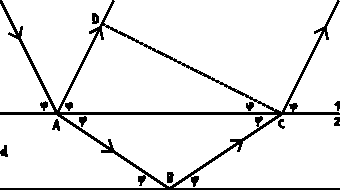
\includegraphics[width=0.55\textwidth]{content/graphics/kiessig.pdf}
	\caption{Schematic light paths inside a thin layer atop a substrate producing Kiessig oscillations according to \cite{Kiessig_1931}.}
	\label{fig:kiessig}
\end{figure}

In the first medium, the waves traverse as distance $AD$ while covering a length $n(AB + BC)$ in the second medium. Their difference is
\begin{equation*}
	\Delta = n(AB + BC) - AD \: .
\end{equation*}
Expressing $AB, BC$ in terms of $d, \psi$ and applying the small angle approximation,
\begin{equation*}
	AB = BC = \pfrac{d}{\sin\psi} \cong \pfrac{d}{\psi}
\end{equation*}
as well as
\begin{equation*}
	AC = (AB + BC)\cos\theta
\end{equation*}
for
\begin{equation*}
	AD = AC\cos\varphi = nAC\cos\psi = \pfrac{2dn\cos^2\psi}{\sin\psi} \cong \pfrac{2dn}{\psi}\cos^2\psi \cong \pfrac{2dn}{\psi} - 2dn\psi
\end{equation*}
follow, where the expansion
\begin{equation*}
	\cos^2\psi \cong 1 - \psi^2
\end{equation*}
is used. One then obtains
\begin{equation*}
	\Delta \cong \pfrac{2dn}{\psi} - \pfrac{2dn}{\psi} + 2dn\psi \cong 2d\psi \: ,
\end{equation*}
where the last step neglects products of $\delta, \beta, \psi \ll 1$. Using \eqref{eqn:angles},
\begin{equation*}
	\Delta \cong 2d\sqrt{\varphi^2 - 2\delta \pm 2i\beta} \: ,
\end{equation*}
which produces an interference minimum for $\Delta = m\lambda$ with $m \in \mathbb{Z}$ and the wavelength $\lambda$.
When comparing minima,
\begin{equation*}
	m_{1, 2}\lambda \equiv 2d\sqrt{\varphi_{1, 2}^2 - 2\delta \pm 2i\beta}
\end{equation*}
and by subtracting, rearranging and inserting, one arrives at
\begin{align*}
	d = \pfrac{\lambda}{2} \sqrt{\pfrac{m_1^2 - m_2^2}{\varphi_1^2 - \varphi_2^2}} \: , &&
	\delta = \pfrac{m_1^2 \varphi_2^2 - m_2^2 \varphi_1^2}{2 (m_1^2 - m_2^2)}
\end{align*}
for the thickness $d$ and real refractive correction $\delta.$ In the case of adjacent minima,
\begin{equation}
	d \cong \pfrac{\lambda}{2(\varphi_1 - \varphi_2)}
	\label{eqn:thick}
\end{equation}
serves as a reasonable approximation.



\subsection{Stratified media}

When considering the reflectivity of multiple homogenous layers with sharp boundaries, the transmission and reflection of all lower layers
has to be taken into account. To do so, Parratt introduced an exact recursive formalism \cite{Parratt_1954}. This assumes an infinite substrate
and surrounding medium, allowing one to start with simple Fresnel reflectivity at the very bottom layer before iterating up towards the surface
as sketched in Figure \ref{fig:parratt}.

\begin{figure}[H]
	\centering
	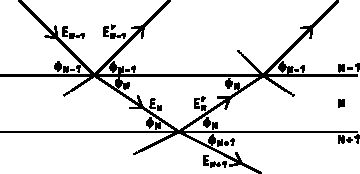
\includegraphics[width=0.55\textwidth]{content/graphics/parratt.pdf}
	\caption{Conceptual visualization of the Parratt algorithm presented in \cite{Parratt_1954}.}
	\label{fig:parratt}
\end{figure}

The wave vector $n_j^2 k^2 = k_j^2 = k_{j, x}^2 + k_{j, z}^2$ in combination with the continuity of the tangential component $k_{j, x} = k_x$
can be used to write
\begin{equation*}
	k_{j, z}^2 = n_j^2 k^2 - k_{j, x}^2 = n_j^2 k^2 - k_x^2 = (1 - \delta_j \pm i\beta_j)^2 k^2 - k_x^2 \cong
	(1 - 2\delta_j \pm 2i\beta_j) k^2 - k_x^2\: ,
\end{equation*}
where the last step neglects products of $\delta_j , \beta_j \ll 1$, leading to
\begin{equation*}
	k_{j, z} \cong \sqrt{k_z^2 - 2\delta_j k^2 \pm 2i\beta_j k^2} \: .
\end{equation*}
Further, one identifies $k_z = k \sin\alpha_i \cong k \alpha_i$ for
\begin{equation}
	k_{j, z} \cong k \sqrt{\alpha_i^2 - 2\delta_j \pm 2i\beta_j} \: ,
	\label{eqn:kz}
\end{equation}
analogous to the result from \eqref{eqn:angles}. Adopting the conventions in \cite{Schreiber_2004, Tolan_1999}, Fresnel's coefficients
can be written as
\begin{equation}
	r_{j, j + 1} = \pfrac{k_{j, z} - k_{j + 1, z}}{k_{j, z} + k_{j + 1, z}}
	\label{eqn:fresnel-kz}
\end{equation}
at the boundary between layers $j$ and $j+1$. With this, the Parratt algorithm reads
\begin{equation}
	x_j = \pfrac{r_j}{t_j} = e^{-2i k_{j, z} d_j} \pfrac{r_{j, j + 1} + x_{j + 1} e^{2i k_{j + 1, z} d_j}}
	{1 + r_{j, j + 1} x_{j + 1} e^{2i k_{j + 1, z} d_j}} \: ,
	\label{eqn:parratt}
\end{equation}
which for $N$ layers has starting parameters $x_{N + 1} = r_{N + 1} = 0$ since there are no reflections from the infinte substrate
$N + 1$ and $t_0 = 1$ as the normalization of the incident ray in the surrounding air or vacuum. The intensity reflectivity is obtained
via $R = |r_0|^2 = |x_0|^2$. Accounting for rough boundaries, the specular Fresnel factors are modified such that
\begin{equation}
	r_{j, j + 1} \rightarrow r_{j, j + 1} e^{-2 k_{j, z} k_{j + 1, z} \sigma_{j, j + 1}^2},
	\label{eqn:roughness}
\end{equation}
where deviations following an uncorrelated Gaussian distribution much smaller than the layer thickness $d_j$ are assumed and the roughness
is measured by $\sigma_{j, j + 1}$.



\subsection{Geometry factor}

At low glancing angles $\alpha_i$, the beam width $\tilde{d}$ exceeds the effective size $D \sin\alpha_i$ of the sample, meaning the reflected
intensity no longer corresponds to the full beam as shown in Figure \ref{fig:geometry}. Correcting for this, the intensity $I$ is divided by the
geometry factor
\begin{equation}
	G = \left\{ \begin{array}{ll} \pfrac{D \sin\alpha_i}{\tilde{d}} & \alpha_i < \alpha_g \\ 1 & \alpha_i \geq \alpha_g \\ \end{array} \right.
	\label{eqn:geom-factor}
\end{equation}
as $I \rightarrow I / G$, with the geometry angle defined by $\tilde{d} = D\sin\alpha_i \cong D\alpha_g$ or
\begin{equation}
	\alpha_g \cong \pfrac{\tilde{d}}{D} \: .
	\label{eqn:geom-angle}
\end{equation}

\begin{figure}[H]
	\centering
	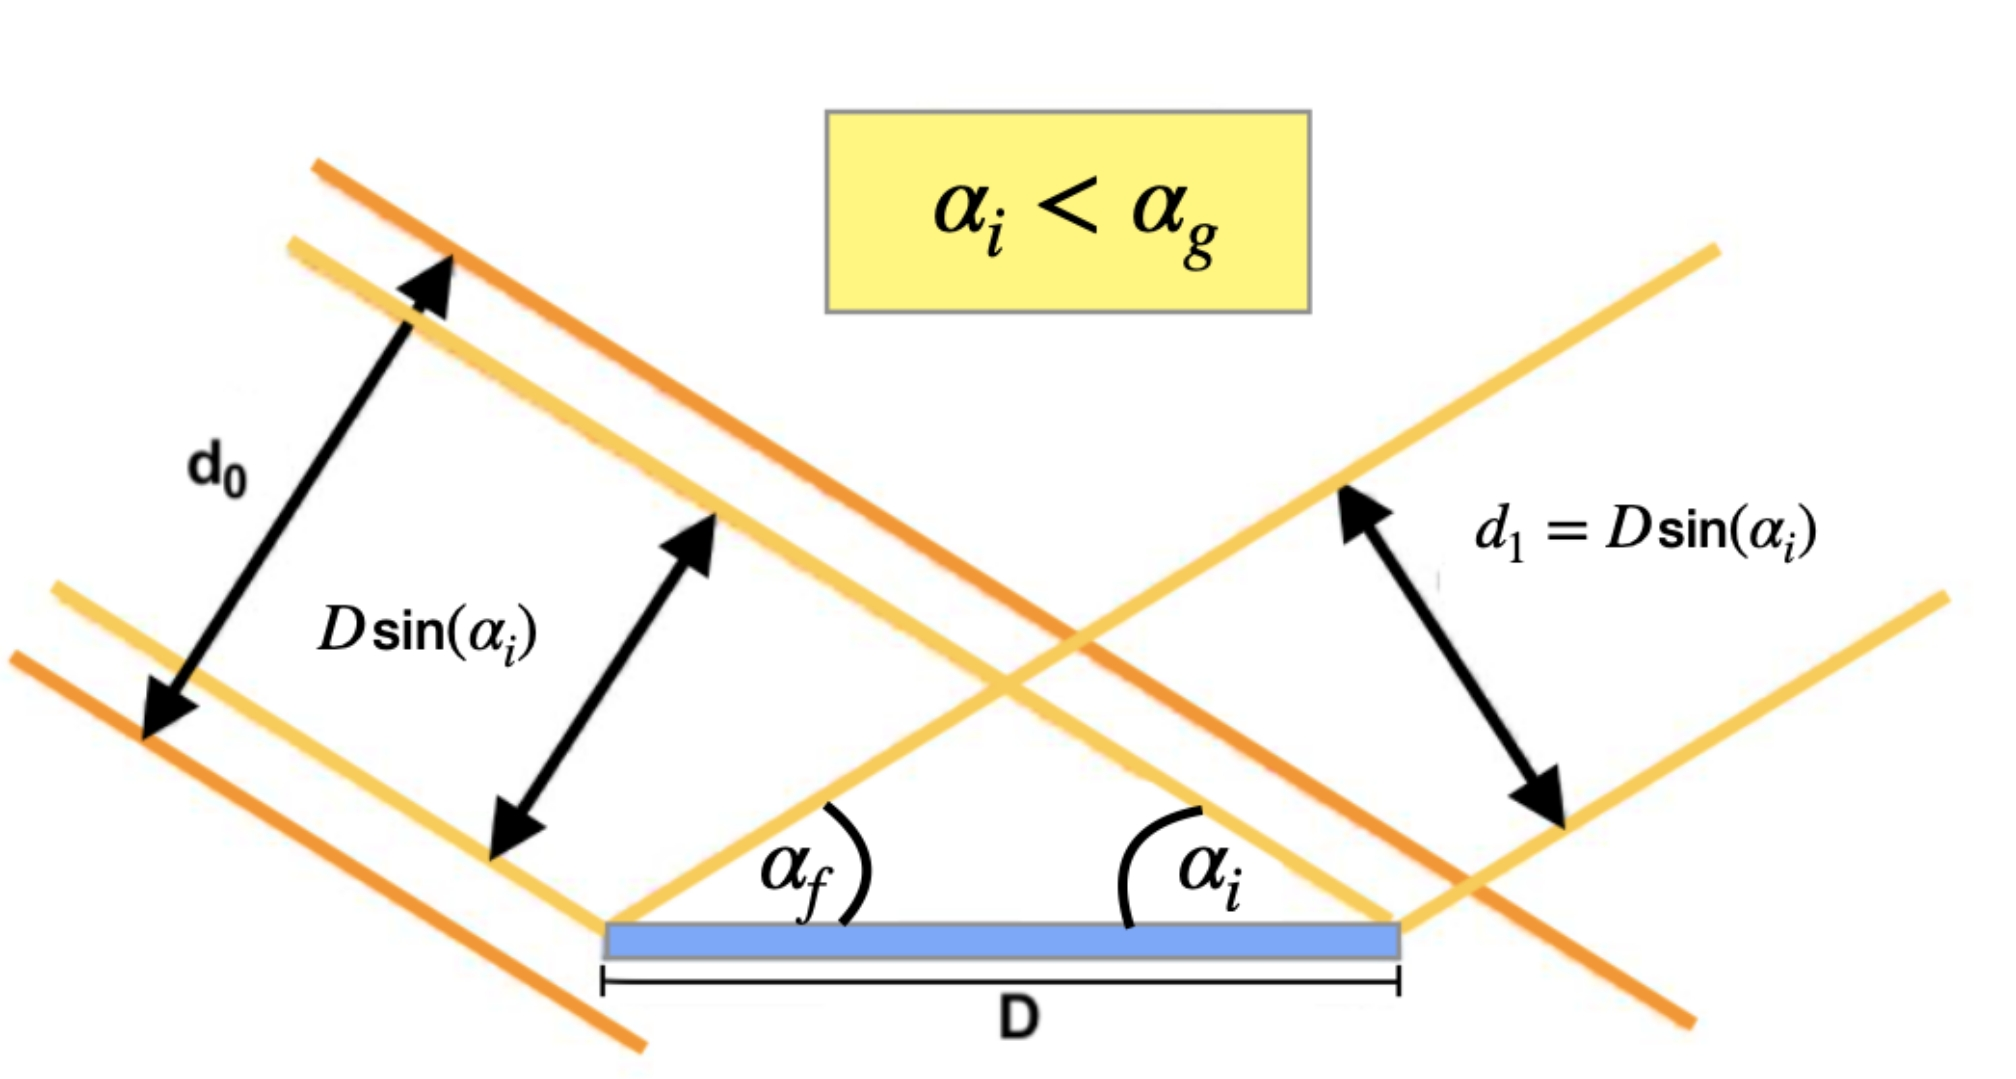
\includegraphics[width=0.66\textwidth]{content/graphics/geometry.jpg}
	\caption{Beam geometry for partial obstruction by the sample at low angles \cite{xray}.}
	\label{fig:geometry}
\end{figure}
